\section{Durchführung}
\label{sec:Durchführung}

Für die Versuchsdurchführung wird die Apparatur in \autoref{fig:messapparatur} verwendet.
Sie besteht hauptsächlich aus einer Kupfer-Röntgenröhre, einem LiF-Kristall bzw. hier einen Plexiglas-Streuer und einem Geiger-Müller-Zählrohr.
Der Versuch kann über einen Rechner verlaufen.
Hierfür wird am PC das Programm measure genutzt.
Bei jedem Versuchsteil wird die Messart, der Drehmodus, der anzufahrende Kristallwinkel und die Integrationszeit eingestellt.
Die Beschleunigungsspannung beträgt bei allen Messungen $\SI{35}{\kilo\volt}$ und der Emissionsstrom $\SI{1}{\milli\ampere}$.

\begin{figure}
    \centering
    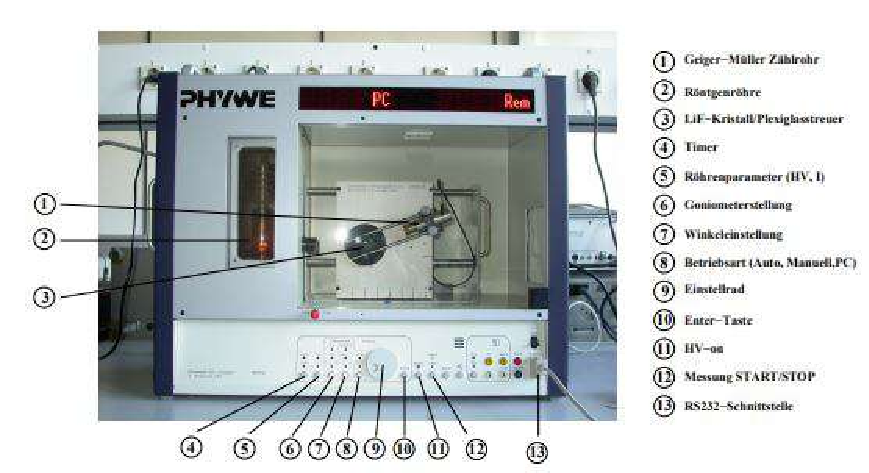
\includegraphics[width=\textwidth]{bilder/messaparatur.pdf}
    \caption{Die Messaparatur bestehend aus einer Kupfer-Röntgenröhre, einem LiF-Kristall bzw.
            einem Plexiglas-Streuer und einem Geiger-Müller-Zählrohr. \cite{anleitung} }
    \label{fig:messapparatur}
\end{figure}

\subsection{Aufnahme eines Emissionsspektrums der Kupfer-Röntgenröhre}
Eine $\SI{2}{\milli\metre}$ Blende und ein LiF-Kristall werden hier verwendet.
Das Emissionsspektrum wird nun aufgenommen indem der Winkel des LiF-Kristalls um $\increment \alpha = 0.1°$ und mit einer Integrationszeit von $t=\SI{10}{\second}$ variiert wird.

\subsection{Bestimmung der Transmission als Funktion der Wellenlänge}
Der Aluminium-Absorber $N_\text{Al}$ wird vor die $\SI{2}{\milli\metre}$ Blende gesetzt.
Die Zählrate der Röntgenstrahlung wird nun gemessen, dabei befindet sich der Kristallwinkel in einem Winkelbereich von $\alpha = [7°,10°]$.
Dieser Kristallwinkel wird in $\increment \alpha = 0.1°$ Schritten und einer Integrationszeit von $t = \SI{200}{\second}$ verändert.
Dieselbe Messung wird ohne Aluminium-Absorber $N_0$ wiederholt.

\noindent Es folgt eine Korrektur der gemessenen Zählrate mit der Totzeit $\tau = \SI{90}{\micro\second}$ des Geiger-Müller Zählrohrs:
\begin{equation}\label{eqn:korrektur}
    I = \frac{N}{1 - \tau \cdot N} \, ,
\end{equation}
hierbei steht I wiederum für eine Zählrate.\\

\noindent
Im weiteren Versuchsdurchlauf wird eine manuelle Messung durchgeführt.
Hierzu wird das RS232-Kabel entfernt und das Röntgengerät auf Manuell gestellt.
Die vorzunehmenen Einstellungen erfolgen am Einstellknopf, siehe \autoref{fig:messapparatur} und werden mit ENTER bestätigt.
Oben an der Messaparatur befindet sich eine Anzeige zum Ablesen der gemessenen Zählrate.

\subsection{Bestimmung der Compton-Wellenlänge}
Die Transmission der ungestreuten und gestreuten Röntgenstrahlung soll untersucht werden.
Hierzu wird die $\SI{2}{\milli\metre}$ Blende durch eine $\SI{5}{\milli\metre}$ Blende ersetzt.
Zudem wird der LiF-Kristall mit einen Plexiglas-Streuer ausgetauscht.
Der Streuer wird auf 45° und das Geiger-Müller-Zählrohr auf 90° gesetzt, siehe \autoref{fig:plexiglas}.
Nun wird die Intensität $I_0$ der Kupfer-Röhre gemessen. \\
\noindent
Zunächst wird die Transmission $T_1$ der ungestreuten Röntgenstrahlung betrachtet.
Wie in \autoref{fig:plexiglas}a zu sehen, wird der Aluminium-Absorber in den Strahlengang zwischen Röntgen und Streuer gesetzt. \\
\noindent
Um die Transmission $T_2$ der gestreuten Röntgenstrahlung zu untersuchen, wird der Aluminium-Absorber in den Strahlengang zwischen Streukörper und Geiger-Müller-Zählrohr gebracht,
siehe \autoref{fig:plexiglas}b. \\
Die Integrationszeit beträgt $t = \SI{300}{\second}$.
Die Zählraten werden notiert.

\begin{figure}
    \centering
    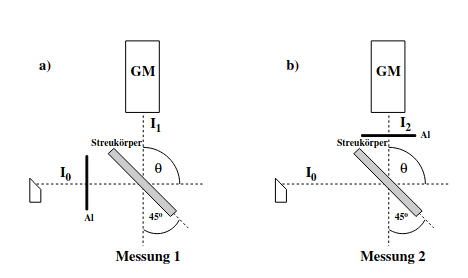
\includegraphics[width=0.7\textwidth]{bilder/plexiglas_aufbau.png}
    \caption{Der experimentelle Aufbau der Messung mit dem Plexiglasstreuer. \cite{anleitung} }
    \label{fig:plexiglas}
\end{figure}